\section{Introduction}

This thesis addresses the following research question \enquote{What can mixed-method social network analysis reveal about tacit knowledge sharing behaviour in open innovation?}. Not much is known about tacit knowledge in open innovation. This gap in understanding may be attributed to tacit knowledge being a messy concept that is usually job-specific, difficult to study, and often regarded as being of negligible epistemic worth \citep{mohajan2016sharing}. \medskip

Open innovation is defined as \enquote{a distributed innovation process based on purposively managed knowledge flows across organisational boundaries} \citep{chesbrough2014explicating}. This definition considers knowledge in terms of the \enquote{epistemology of possession}. The epistemology of possession treats knowledge as something people possess (know-what or know-that), whereas the epistemology of practice refers to knowing how to enact knowledge in practice (know-how) \citep{cook1999bridging}. Although there are many aspects to managing knowledge flows across organisational boundaries, this thesis argues that open innovation is mainly about facilitating the interaction between know-how (practical knowledge on how to accomplish something) and know-what (factual knowledge) \citep{winter1987knowledge, garud1997distinction}.  \medskip

This chapter explores the epistemology of knowledge and examines how tacit knowledge can facilitate innovation. Moreover, because tacit knowledge is not easily shared or readily given up, this chapter also looks at psychological and social factors that potentially shape tacit knowledge sharing behaviour. It conceptualises an open innovation partnership as a temporary knowledge network deliberately set up to achieve a specific innovation outcome within a market-relevant time frame. Embracing a network perspective offers valuable insights into the self-organising (endogenous) and external (exogenous) factors influencing tacit knowledge transfer processes. \medskip

Agency is vital because it lies at the heart of tacit knowledge sharing \citep{polanyi1966tacit}. It is what drives the emergence of informal structures that allow know-how and know-what to come together \citep{lam2014tacit, hubrich2015embodiment}. The extent to which structure inhibits or encourages agency in open innovation has not received much attention in the literature so far. Structure refers to the patterned arrangements that influence or limit the choices and opportunities available to individuals \citep{bandura1999social}. Too much structure may inhibit participants' willingness to share tacit knowledge or contribute ideas \citep{lam2000tacit}. Conversely, too little structure can make goals less clear, leading to unsatisfactory open innovation outcomes. Finding the right balance between structure and agency is considered essential for successful open innovation \citep{davis2010agency}. \medskip

This chapter formulates several propositions about tacit knowledge sharing in open innovation. As this study is exploratory, the propositions are less about testing specific hypotheses about tacit knowledge sharing than gaining a deeper and more nuanced understanding of tacit knowledge sharing behaviour in open innovation. The propositions serve as signposts for exploratory research.

\section{The nature of knowledge}

Given this thesis is about tacit knowledge sharing, it is prudent to consider the epistemology of knowledge before venturing further. Traditionally, knowledge is considered a justified true belief \citep{bolisani2018elusive}. For those who embrace a positivist worldview, truthfulness is the main feature of knowledge. Positivists see knowledge as objective, static, and absolute. Others who embrace a constructivist or pragmatic worldview, place more weight on justified beliefs. For them, the utility of knowledge is more important than truthfulness \citep{bolisani2018elusive}. \citet{spender1996organizational} observes that \enquote{knowledge is less about truth and reason and more about the practice of intervening knowledgeably and purposefully in the world}. What matters is not what we know, but knowing how to apply our knowledge \citep{ryle1949concept,orlikowski2002knowing}. \medskip

It is helpful to think about how people know things. Two perspectives dominate the theory of knowledge: rationalism and empiricism. Rationalism argues that knowledge is the result of a reasoning process. Knowledge exists in our minds. What is observed or sensed does not constitute knowledge \citep{russell2009human}. On the other hand, empiricism argues that knowledge is a product of our sensory interface with the real world \citep{bolisani2018elusive}. The distinction between rationalism and empiricism becomes useful when interpreted to mean that humans know in two ways, either through experience or reasoning. When these two ways of knowing interact, new knowledge is often created \citep{spender1996making,bolisani2018elusive}. \citet{cook1999bridging} consider knowledge in terms of the epistemology of possession and the epistemology of practice. The epistemology of possession treats knowledge as something people possess (know-what or know-that), whereas the epistemology of practice refers to knowing how to enact knowledge in practice (know-how). Know-how is the ability to put know-what into practice \citep{cook1999bridging,tsoukas2001organizational, marabelli2014knowing}. \medskip

\citet{polanyi1966tacit} states that people often know how to do things by adhering to a set of rules they are unaware of. He refers to this unknown set of rules for skillful action as tacit knowledge (or tacit knowing, to be more precise). People accumulate tacit knowledge through observation, imitation, and repeated interaction. Tacit knowledge is deeply rooted in personal experience \citep{nonaka1995knowledge}. Not only is tacit knowledge embodied in the minds and actions of individuals, but it is also manifest in group practice and culture, usually in the form of unwritten rules and procedures \citep{munoz2015tacit}. \medskip

Innovation is about transforming ideas into reality, a process that involves applying know-how to new or existing knowledge in novel ways \citep{van1986central,quintane2011innovation,garud2013perspectives}. This perspective implies that open innovation is more about creating the social conditions that allow know-how and know-what to come together than simply managing knowledge flows. Sharing know-how enables others to learn the practice that entails the know-how \citep{van1986central,goksel2016can}.

\section{Knowledge networks}

As stated earlier, this thesis considers an open innovation partnership to be temporary knowledge network set up deliver some form of innovation. A knowledge network connects individual and organisational actors across organisational, spatial, and disciplinary boundaries to create, share, or apply a body of knowledge \citep{pugh2013designing}. Some researchers distinguish between a knowledge network and a social network \citep[e.g.][]{yayavaram2008decomposability,wang2014knowledge,brennecke2017firm}. Such a distinction is warranted if one treats people and knowledge as separable entities. As tacit knowledge is embodied in the minds and actions of people, such a distinction is not appropriate for this thesis. Instead, the thesis treats a knowledge network as a social network, where ties represent social interactions between knowledgeable actors. Embracing a network perspective offers valuable insights into the self-organising (endogenous) and external (exogenous) factors influencing tacit knowledge transfer processes. \medskip

The value a firm can extract from its knowledge network depends on the reach of the firm's ties to diverse and distant partners, the richness of knowledge embedded in the network, and how easily a firm can harness network resources \citep{gulati2011networks}. We can describe a firm's reach in terms of its weak knowledge ties \citep{hansen1999search}. Actors connected by strong ties often share similar interests and are privy to the same knowledge. Strong ties tend to make people look inward and be less receptive to external knowledge. Actors connected by weak ties tend to mix in different social circles and are thus more exposed to different knowledge and opportunities \citep{granovetter1973strength}. \medskip

Regarding the richness of knowledge resources, the depth of knowledge and quality of knowledge is of primary importance, as this determines the potential value of the knowledge resource \citep{davenport1998working,kane2005knowledge}. The depth of knowledge reflects its usefulness for problem-solving. Addressing simple problems requires basic know-how. As problems become increasingly complex, higher levels of cognition are required. More profound know-how is required to solve increasingly challenging problems \citep{webb2002depth,bennet2008depth}. We can describe the quality of knowledge in terms of its usability, completeness, currency, and accuracy \citep{wixom2005theoretical}. \medskip

When examining the structure of a knowledge network, a \enquote{structural hole} refers to gaps between separate groups of people \citep{burt2000network}. Groups on either side of the structural hole are privy to different knowledge. Members of tightly knit groups are more likely to work with tacit knowledge in the form of mutually understood, unwritten language and routines to coordinate with one another \citep{burt2007secondhand}. Structural holes present an opportunity to broker knowledge exchanges between otherwise disconnected groups of people. A knowledge network with an abundance of structural holes facilitates innovation by allowing strategically placed actors to access and combine diverse knowledge in novel ways \citep{burt2004structural,sparrowe2011publishing}. \medskip

Because tacit knowledge familiar within groups is likely to be invisible to other groups, it can yield a premium to brokers who coordinate such knowledge across the groups \citep{burt2007secondhand}. While brokerage across structural holes in a disconnected knowledge network is the source of value, network closure is critical to realising the value buried in structural holes \citep{burt2004structural,rost2011strength}. Network closure refers to a human tendency to form into social groups (see Figure \ref{fig:closure}). More closed networks with fewer structural holes promote trust and reduce opportunism, leading to more productive collaboration from knowledge sharing \citep{ahuja2000collaboration, burt2007secondhand}. \medskip

In summary, we conceive an open innovation partnership as a temporary knowledge network set up to achieve a specific innovation outcome. This thesis considers knowledge in terms of the \enquote{epistemology of practice}. Extracting value from a knowledge network depends on individuals being able to gain access to relevant knowledge embedded in the network and their ability to leverage this knowledge. While connections across structural holes are a source of value in a knowledge network, network closure is vital for realising the value buried in structural holes.  Open innovation is mainly about facilitating the interaction between know-how (practical knowledge on how to accomplish something) and know-what (factual knowledge) \citep{winter1987knowledge,garud1997distinction}. Sharing know-how enables others to learn the practice that entails the know-how. Hence, \bigskip

\begin{tcolorbox}
\textit{\textbf{Proposition 1a:} Open  innovation  requires  practitioners  to  connect across organisational and disciplinary boundaries so that they can apply their know-how in novel ways.}
\end{tcolorbox}

\section{Absorptive capacity} 

This section reviews the concept of absorptive capacity and what this means in terms of tacit knowledge sharing in open innovation. Thus far, we have examined capturing value from temporary knowledge networks by bridging structural holes and achieving network closure. How easily open innovation partners can harness knowledge embedded in a network depends on several factors. Complex knowledge usually has a significant tacit component to it. Transferring complex knowledge is difficult because it involves transferring relevant know-how between partners as well. The human dimension of complex knowledge makes it particularly \enquote{sticky} \citep{von1994sticky,szulanski2003sticky}. Absorptive capacity is the ability of a firm to recognise, acquire, assimilate, transform, and exploit new external knowledge \citep{cohen1990absorptive}. Relative differences in absorptive capacity between open innovation partners can also impede efforts to combine or integrate different ways of knowing \citep{vanhaverbeke2007connecting,lichtenthaler2016absorptive}. Despite being the subject of countless studies, the extent to which absorptive capacity contributes to a firm's innovation performance is still an open issue \citep{omidvar2013revisiting,duchek2013capturing}. \medskip

What is absorptive capacity exactly? \citet{cohen1990absorptive} embrace a cognitive approach to absorptive capacity by connecting ideas from individual learning to organisations. The amount of experiential knowledge a firm can accumulate through its employees determines its absorptive capacity. In other words, tacit knowledge is a component of absorptive capacity. \citet{cohen1990absorptive} view the relationship between absorptive capacity and the level of experiential knowledge as a positive feedback loop, where an increase in absorptive capacity improves the level of relevant knowledge, which in turn further increases absorptive capacity. Mediating this feedback loop is the environment the firm operates in \citep{van1999coevolution}. \citet{lane1998relative} suggest that absorptive capacity is more about the ability of a firm to learn from another. This ability is a function of the extent to which firms have overlapping knowledge bases and the extent to which they socially interact \citep{dyer1998relational,nooteboom2000learning}. \medskip

Early studies paid little attention to the processes that build absorptive capacity leading \citet{zahra2002absorptive} to re-conceptualise absorptive capacity as a dynamic capability that integrates internal processes for acquiring, assimilating, transforming, and exploiting external knowledge. They describe knowledge acquisition as the ability of a firm to identify and acquire externally generated knowledge critical to its operation. Knowledge assimilation encompasses the processes used by a firm to make sense of externally sourced knowledge, whereas knowledge transformation refers to the processes used by a firm to integrate assimilated external knowledge with existing internal knowledge. Knowledge exploitation is about the processes used by a firm to enhance existing competencies or create new ones by incorporating acquired and transformed knowledge into its operations. \citet{zahra2002absorptive} distinguish between potential absorptive capacity, namely the capability to acquire and assimilate new external knowledge, and realised absorptive capacity, which is the capability to transform and exploit knowledge. They suggest that the ratio of realised absorptive capacity to potential absorptive capacity measures the efficiency of an organisation at leveraging absorbed knowledge. \citet{zahra2002absorptive} also highlight the importance of social mechanisms that connect people who acquire external knowledge with people inside the firm who can apply this knowledge. \citet{jansen2005managing} find coordination capabilities, namely brokerage, shared decision-making and job rotation, enhance potential absorptive capacity, whereas socialisation capabilities (indicated by network closure) increase realised absorptive capacity. \medskip

\citet{todorova2007absorptive} highlight how different appropriability mechanisms may influence absorptive capacity. Firms may employ several mechanisms to protect their knowledge from being appropriated by others. How and when these are applied is often unclear and can create tension between knowledge sharing and knowledge protection practices \citep{gama2019managing}. Firms do not want to leak valuable knowledge as quickly as they absorb it \citep{todorova2007absorptive}. Tension between knowledge sharing and knowledge protection can thwart the inter-organisational learning needed to overcome relative differences in absorptive capacity \citep{dragsdahl2019perspective,gama2019managing}. \medskip

\citet {lichtenthaler2016absorptive} argues that past studies have overlooked the negative consequences of building absorptive capacity. These include challenges in capturing value from knowledge, overemphasising prior-related knowledge, and inter-dependencies between internal processes. The challenges around capturing value relate to the capabilities needed to manage increasingly sophisticated knowledge and the rising cost of capability development. \citet{lichtenthaler2016absorptive} claims that firms struggle to capture value from tacit knowledge, and prior-related knowledge may be of limited use when it comes to adapting and transforming knowledge for use in new contexts. Firms may not benefit from externally sourced knowledge because it may decay over time. \medskip

\citet{marabelli2014knowing} interpret a firm's absorptive capacity in terms of the epistemology of possession and the epistemology of practice. They differentiate between knowledge that resides in people's minds, easily spread by individuals who can develop a shared understanding with others and sticky knowledge enacted in practice. The epistemology of practice treats absorptive capacity as a capability that emerges when applying knowledge in practice. \citet{marabelli2014knowing} argue that a practice-based perspective provides a more nuanced perspective of power and how it shapes absorptive capacity. They refer to prohibitive and productive power (also referred to as power-over and power-to, respectively). Prohibitive power focuses on the power of organisational actors to control knowledge and achieve objectives at the expense of others. On the other hand, productive power focuses on empowering (or disempowering) actors to change knowledge practices. \medskip

Open innovation puts the organisational practices used to source and apply external knowledge into sharp focus. Treating an open innovation partnership as a temporary knowledge network opens new avenues to explore practices that build absorptive capacity \citep{vanhaverbeke2007connecting,xia2016unpacking}. Absorptive capacity is essentially a learning capacity \citep{cohen1989innovation, cohen1990absorptive, nooteboom2000learning, lichtenthaler2009absorptive}. Moreover, the leading edge of the firm's learning often is found in the tacit knowledge of its employees \citep{horvath2000working}. Tacit knowledge helps bridge cognitive gaps and thus underpins a firm's absorptive capacity \citep{thomas2021tacit}. Because the epistemology of practice treats absorptive capacity as a capability that emerges when applying knowledge in practice, social interaction is crucial for building absorptive capacity. Social interaction allows immediate feedback to confirm understanding and correct any misinterpretations \citep{haldin2000difficulties,gertler2003tacit,koskinen2003tacit}. Hence, \bigskip

\begin{tcolorbox}
\textit{\textbf{Proposition 1b:} Reducing cognitive distance between open innovation partners requires significant social interaction to support learning and the application of knowledge in practice.}
\end{tcolorbox}

\section{Knowledge brokerage}

Brokerage may be defined as the \enquote{behaviour by which an actor influences, manages, or facilitates interactions between other actors} \citep{obstfeld2014brokerage}. Brokers have an important role to play in open innovation \citep{whelan2011creating,cococcioni2014exploring}. They make connections between those who need knowledge and those who have it, i.e. brokers apply their know-who to connect people with the relevant know-how \citep{davenport1998working}. From a network perspective, brokers bridge structural holes. They can use their position to influence access to knowledge resources through their network of weak ties \citep{burt1992structural,hanneman2005introduction,davis2010agency,simpson2011network,stovel2012brokerage}. From a practice perspective, brokers facilitate the integration and synthesis of knowledge provided by others. Both approaches invoke power, but a critical distinction between them is that brokers in open innovation partnerships are less likely to operate only out of self-interest \citep{lingo2010nexus,marabelli2016strategic}. \medskip

\citet{obstfeld2014brokerage} describe three strategic orientations to brokerage: \enquote{conduit}, \enquote{tertius gaudens}, and \enquote{tertius iungens} brokerage. Conduit brokerage is about a third party who transfers information, knowledge, or resources between two disconnected parties. Essentially, a non-partisan broker mediates rather than moderates the relationship between two others and may help them synthesise new knowledge \citep{simmel1950sociology,grosser2019measuring}. Tertius gaudens refers to \enquote{the third who benefits} \citep{simmel1950sociology}. With tertius gaudens brokerage, the broker aims to gain some form of advantage by exploiting differences between two parties, either by keeping them apart or playing one against another. In contrast, tertius iungens (\enquote{the third who joins}) brokerage is about a third-party who introduces two otherwise disconnected parties to each other and encourages them to collaborate (Table \ref{tab:brokerage}). The contention is that brokerage actions, not network structure, are largely responsible for the beneficial outcomes of brokerage i.e. how people broker \citep{grosser2019measuring}. \medskip

\begin{sidewaystable}
\resizebox{0.9\textwidth}{!}{
\begin{threeparttable}
\footnotesize
\setlength{\tabcolsep}{6pt}
\renewcommand{\arraystretch}{1}
\caption[Strategic brokerage orientations]{Strategic brokerage orientations \citep{obstfeld2014brokerage}.}
\label{tab:brokerage}
\begin{tabular*}{\textwidth}{>{\raggedright}p{5cm}>{\raggedright\arraybackslash}p{6cm}>{\raggedright\arraybackslash}p{6cm}>{\raggedright\arraybackslash}p{6cm}}
\toprule
& \multicolumn{1}{c}{Conduit} & \multicolumn{1}{c}{Tertius Gaudens} & \multicolumn{1}{c}{Tertius Iungens} \\ 
\midrule
& \begin{minipage}{0.2\textwidth} \centering 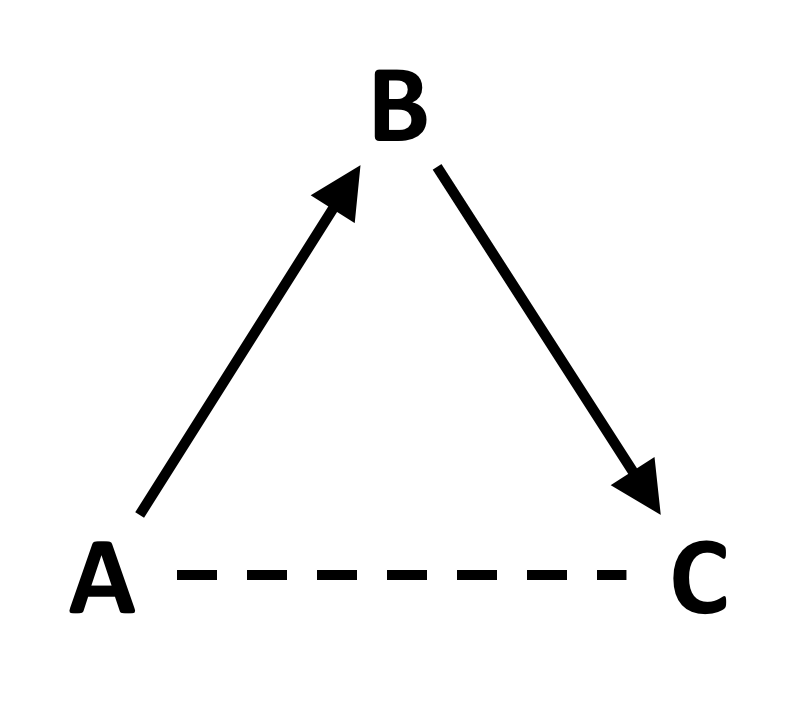
\includegraphics[width=0.7\linewidth]{Images/CDT_brokerage} \end{minipage}  & \begin{minipage}{0.2\textwidth} \centering 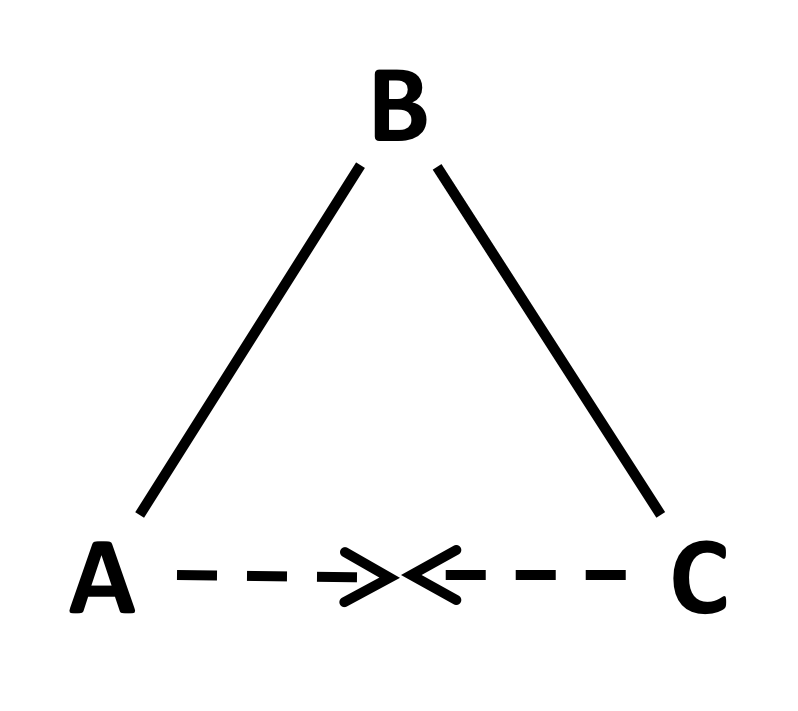
\includegraphics[width=0.7\linewidth]{Images/TG_brokerage_1} \end{minipage}  & \begin{minipage}{0.2\textwidth} \centering 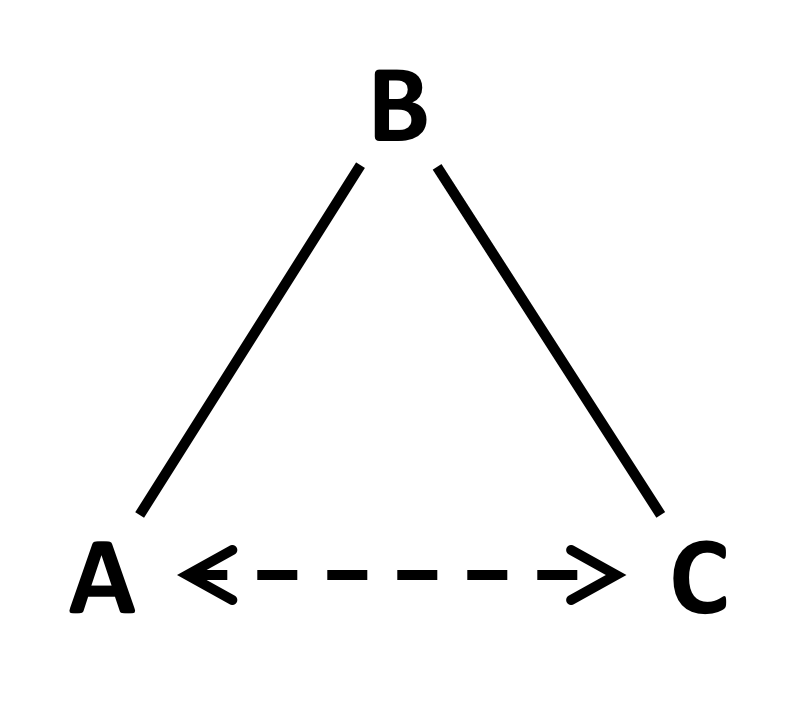
\includegraphics[width=0.7\linewidth]{Images/TI_brokerage} \end{minipage}   \\
&  & \begin{minipage}{0.2\textwidth} \centering 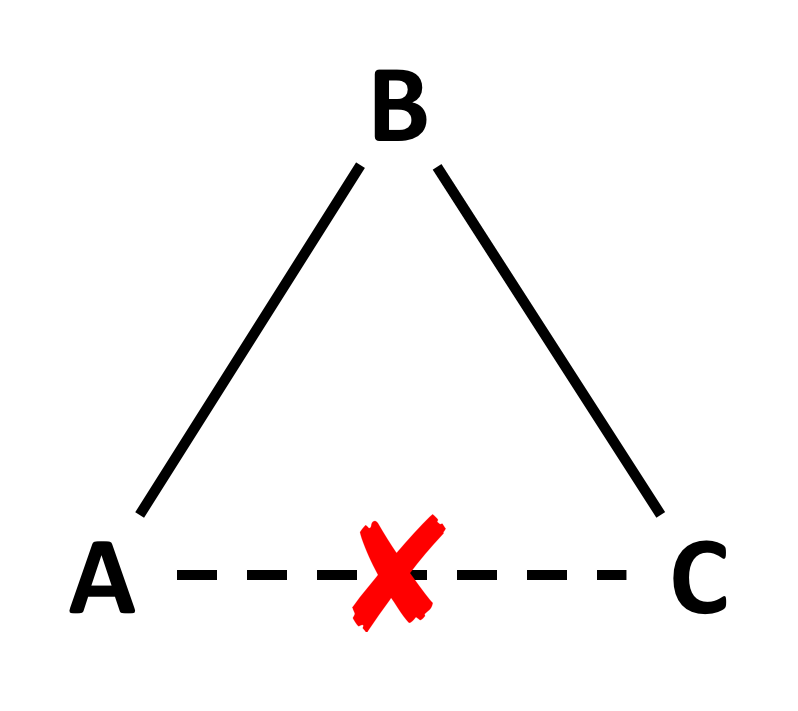
\includegraphics[width=0.7\linewidth]{Images/TG_brokerage_2} \end{minipage}  & \\
\midrule
Open network\\(absence of A-C tie) & B transfers information, knowledge, or other resources between A and C, where A and C have no prospect of meeting. & B plays A and C against one another or keeps A and C apart. & B introduces A and C where A and C have no prior tie. \\
\midrule
Closed Network\\(presence of A-C tie) & B facilitates transfer between A and C and may help synthesise new knowledge. & B cultivates conflict, competition, or separation between A and C (divide et impera) & B coordinates new collaborative action between A and C.  \\ 
\bottomrule
\end{tabular*}
\end{threeparttable}
}
\end{sidewaystable}

Each orientation expresses a different power dynamic. Whereas tertius gaudens brokerage is about exercising power over others, conduit and tertius iungens brokerage are mostly about empowering others \citep{fleming2007collaborative,obstfeld2014brokerage}. Strategic brokerage often involves the selective deployment of these approaches with different actors or for different objectives. Different combinations of tertius iungens and tertius gaudens behaviour are necessary to tailor brokerage strategies to match the situation \citep{lingo2010nexus,obstfeld2014brokerage,quintane2016brokers}. \medskip

The capacity to collaborate with others on complex problems requires relational expertise \citep{edwards2017working}. Such expertise enables joint interpretation of the problem as well as a coordinated response. Knowing how to recognise the expertise of others and being able to demonstrate one's own expertise is crucial. Relational expertise involves recognising the meanings that different practices give to words and how this affects discourse. People with relational expertise are likely to be highly effective knowledge brokers \citep{grigoriou2014structural, edwards2017working}. \medskip

Brokerage is also transient. The ability to engage in tertius gaudens brokerage diminishes when other actors engage in balancing operations to avoid or side-step power-dependencies \citep{emerson1962power}. Likewise, once a broker has introduced one actor to another through conduit or tertius iungens brokerage, their job of empowering others is complete \citep{obstfeld2014brokerage}. However, brokers may sustain tertius iungens brokerage in some coordination or project management role \citep{grosser2019measuring}. Brokers who have outlived their usefulness in a particular situation often seek out new brokerage opportunities. In that way, brokers drive the expansion and evolution of existing networks \citep{obstfeld2014brokerage,quintane2016brokers}. \medskip

From an open innovation perspective, tertius iungens brokerage is essential, especially in the early stages of collaboration, when many actors do not know fellow collaborators in partner organisations very well \citep{fleming2007collaborative}. Knowledge held by third parties is also likely to be unfamiliar, and brokers help others make sense of it. Once ties have formed through tertius iungens brokerage, conduit brokerage is needed to sustain trust and help synthesise and transform knowledge into novel ideas \citep{quintane2016brokers}. \medskip 

When actors belong to distinct groups, group membership allows one to categorise brokerage into five social roles. Brokers can operate as internal coordinators, as mediators, or in a liaison, representative, gatekeeper role depending on their network position \citep{gould1989structures}. Figure \ref{fig:gf_roles} depicts the network configuration of each role. The breakdown of broker roles should provide interesting insights into the character of an open innovation partnership \citep{spiro2013extended}. For example, a partner heavily invested in gatekeeping is likely to be more interested in empowering themselves at the expense of others in the partnership. Alternatively, partners who operate mostly in a representative or liaison broker role are more likely to be invested in the partnership and inclined to empower others \citep{spiro2013extended}. \medskip

\begin{figure}
\centering
  \begin{subfigure}[b]{0.25\textwidth}
    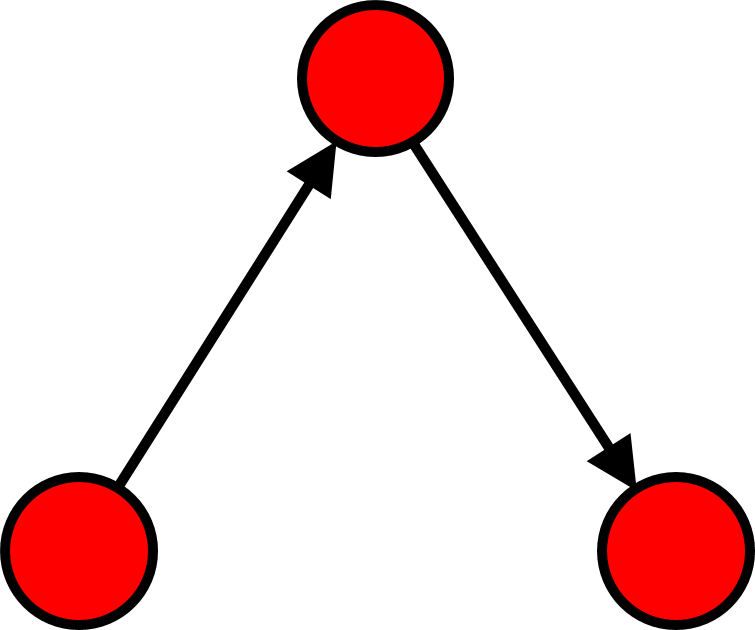
\includegraphics[width=\textwidth]{Images/w_I.png}
    \caption{Coordinator ($w_I$)}
    \label{fig:1}
  \end{subfigure}
  \hspace{2em}
  \begin{subfigure}[b]{0.25\textwidth}
    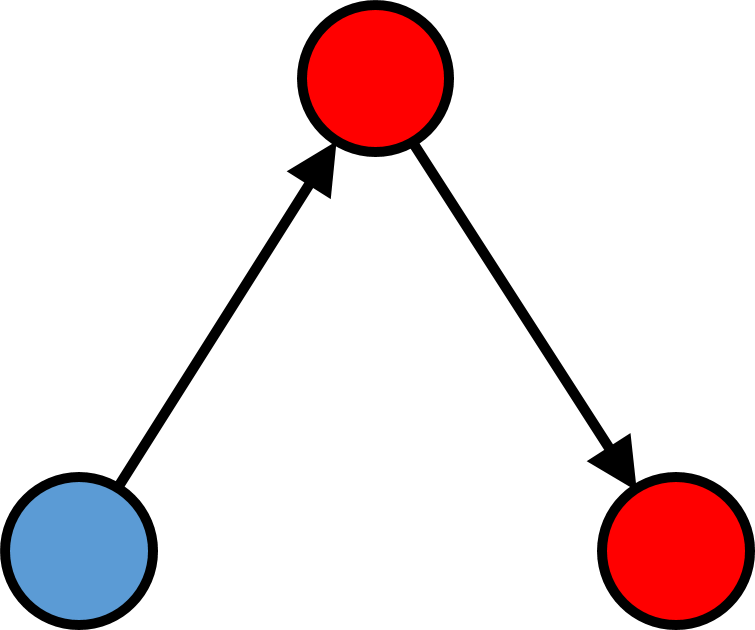
\includegraphics[width=\textwidth]{Images/b_OI.png}
    \caption{Gatekeeper ($b_{OI}$)}
    \label{fig:2}
  \end{subfigure}
  \hspace{2em}
  \begin{subfigure}[b]{0.25\textwidth}
    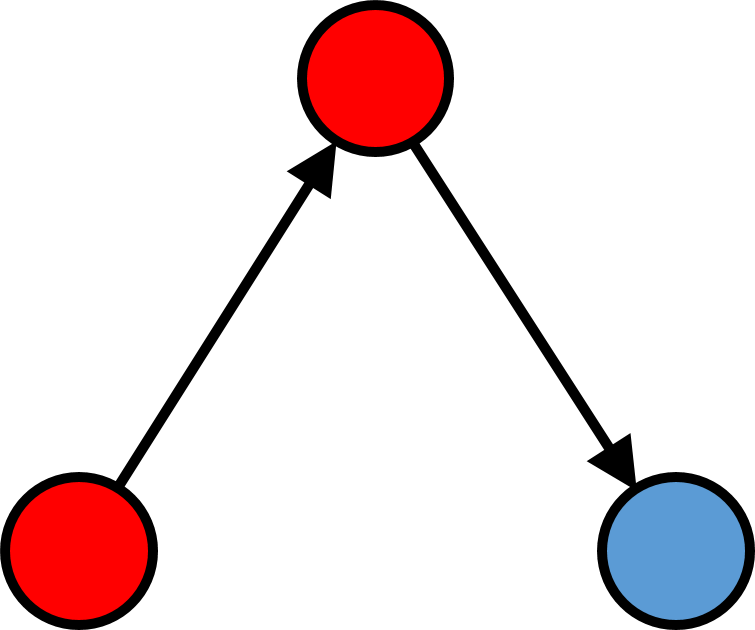
\includegraphics[width=\textwidth]{Images/b_IO.png}
    \caption{Representative ($b_{IO}$)}
    \label{fig:3}
  \end{subfigure}
  \par \bigskip
  \begin{subfigure}[b]{0.25\textwidth}
    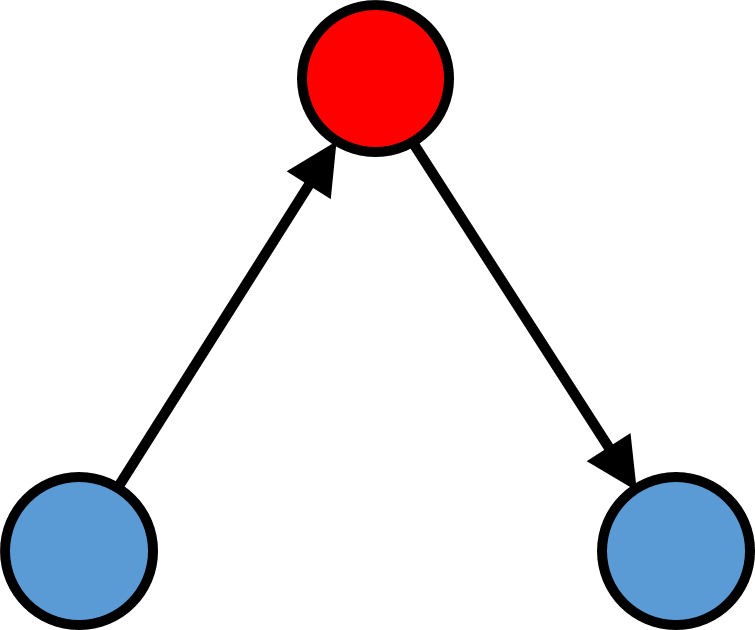
\includegraphics[width=\textwidth]{Images/w_O.png}
    \caption{Mediator ($w_O$)}
    \label{fig:4}
  \end{subfigure}
  \hspace{2em}
  \begin{subfigure}[b]{0.25\textwidth}
    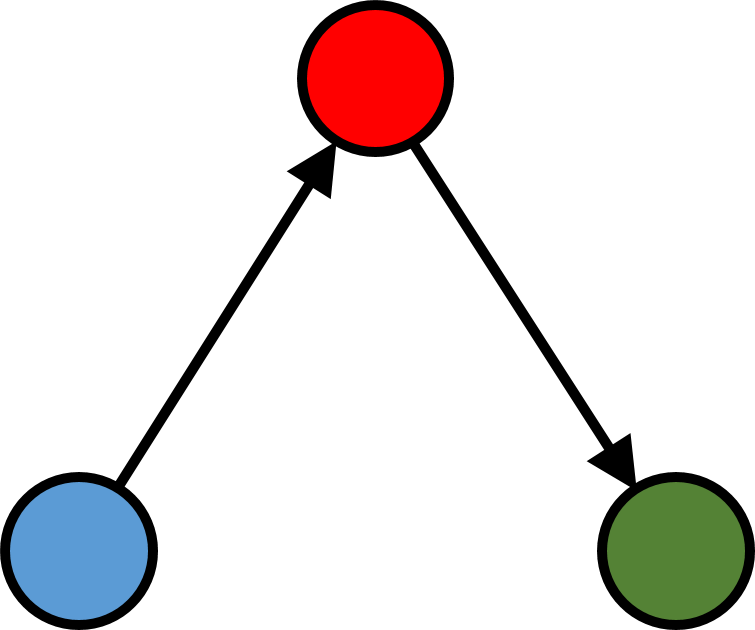
\includegraphics[width=\textwidth]{Images/b_O.png}
    \caption{Liaison ($b_O$)}
    \label{fig:5}
  \end{subfigure}
  \caption[Broker roles]{\citet{gould1989structures} broker roles. The broker is the person receiving and sending ties. Colours represent different group affiliations.}%
    \label{fig:gf_roles}%
\end{figure}

Wrapping up, brokers play a vital role in establishing and growing knowledge networks. They are instrumental in identifying valuable sources of knowledge and connecting people who need knowledge with those who have it. Brokers also help others understand unfamiliar knowledge. From a structural perspective, brokers can use their position to their advantage (tertius gaudens brokerage). Brokers oversee collaborative efforts to integrate and synthesise knowledge to obtain both individual and mutual benefit (tertius iungens and conduit brokerage). Bringing know-how and know-what together to jointly solve problems requires relational expertise. Hence, \bigskip  

\begin{tcolorbox}
\textit{\textbf{Proposition 2a:} Successful open innovation requires a combination of skilled brokerage that leads to network closure.}
\end{tcolorbox}

\section{The structure versus agency debate}

Open innovation requires people to work effectively across organisational and disciplinary boundaries. Working effectively across boundaries requires practitioners to possess good relational skills \citep{chesbrough2012open}. A strong sense of agency is crucial for relational work \citep{edwards2017working}. Agency refers to the capacity to make intentional choices, to initiate actions based on these choices, and to exercise control over oneself and the environment \citep{goller2017human}. Practitioners need to recognise what motivates potential collaborators and make their practice explicit so that others can engage with it \citep{edwards2017working}. Agency drives the emergence of informal structures that allow know-how and know-what to come together \citep{lam2014tacit, hubrich2015embodiment}. \medskip

The structure versus agency debate addresses a fundamental question: do social structures determine how individuals act, or are social structures the product of individual action? There is a growing consensus that structure and agency are complementary. What remains contentious, however, is how these concepts complement each other \citep{tan2011understanding}. According to \citet{giddens1984constitution}, structure is not something external to the individual. He sees structure as patterns of practice. As practices change, so does the structure and vice versa. \citet{giddens1984constitution} uses the term \enquote{duality of structure} to describe structure as both a medium and an outcome. Structure can constrain individual action, but individual action can also transform or create new structures. In other words, structure and agency are deeply entangled or inseparable. The interactions between agency and structure have implications for open innovation. At any particular moment, existing structures constrain and enable agents \citep{emirbayer1998agency}. Their interactions have both intended and unintended consequences that result in the reproduction or transformation of the initial structure. Individual actions contribute to the reinforcement or transformation of the social structure concerned. \medskip

The emerging critical realist perspective of structure versus agency argues that individual action is influenced not just by the causal powers of formal and informal social structures but also by other interacting causal powers, including those of the individual concerned \citep{elder2008searching, elder2010causal,sorrell2018explaining}. In other words, both individuals and social structures have distinctive causal powers that interact to determine social events. Figure \ref{fig:agency_structure} illustrates how causal powers temper need-based actions at both the individual and structural levels. Agency is not a simple matter of having free choice. Instead, it involves making choices that balance individual need dispositions with internalised social norms and social reality \citep{loyal2001agency}. Thus, when considering the structure versus agency debate in open innovation, it is reasonable to assume that structures in each partner organisation influence how individual participants interact across organisational boundaries \citep{llanes2018competitive}. For instance, a partner's appropriability regime can impact inter-organisational knowledge sharing in both positive and negative ways. It may either inhibit knowledge sharing or facilitate knowledge sharing through clearly defined rules of engagement \citep{dahlander2010open,laursen2014paradox,llanes2018competitive}.  \medskip

\begin{figure}[h!]
    \centering
    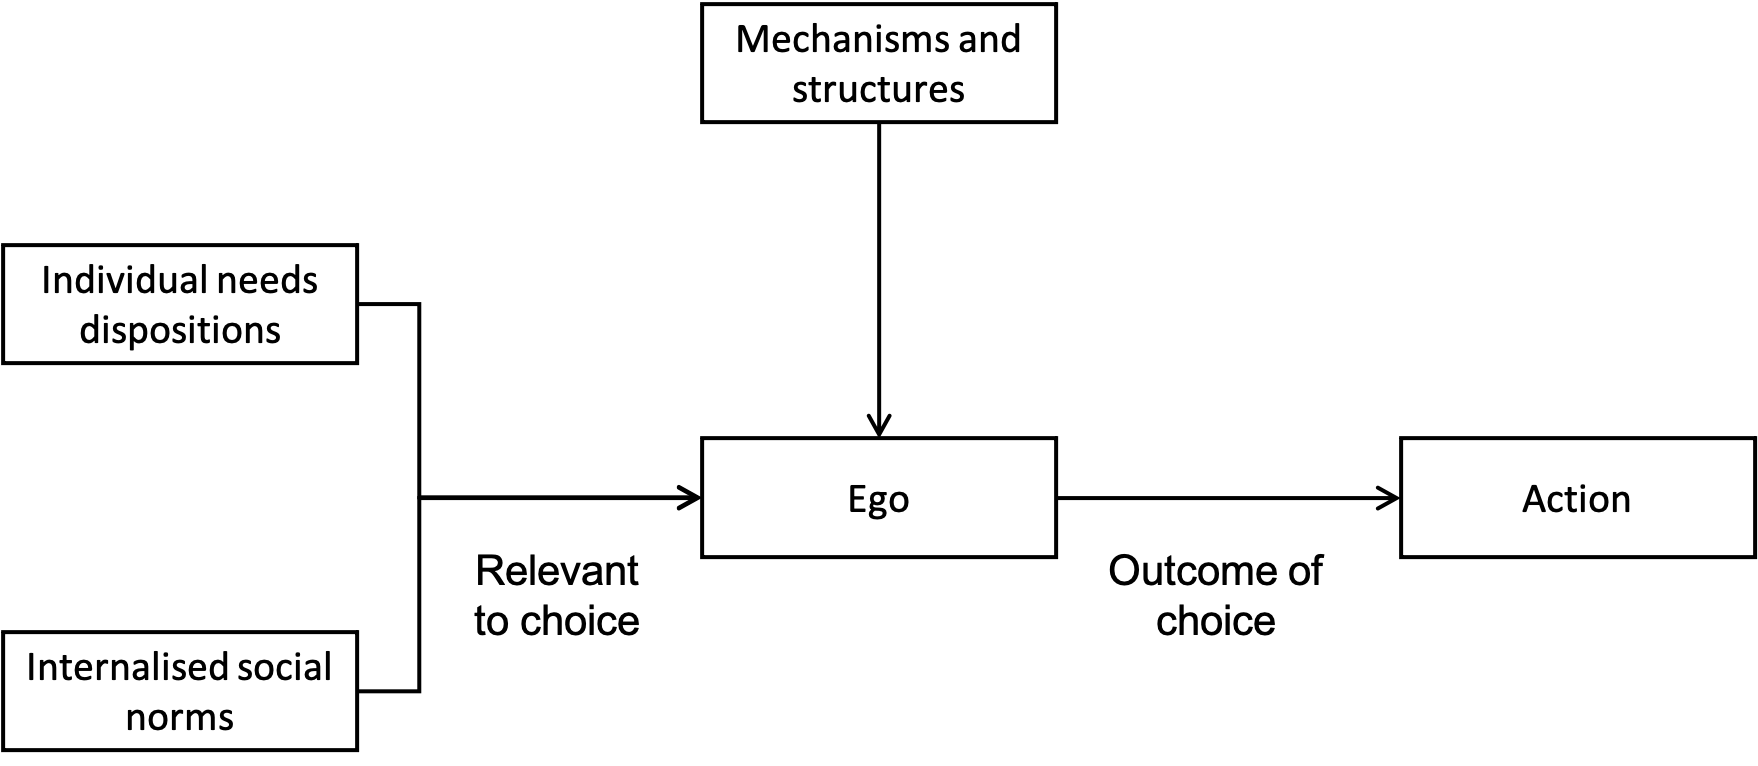
\includegraphics[width=0.9\textwidth]{Images/agency_structure_loyal.png}
    \caption[Critical realist perspective of agency versus structure]{Critical realist perspective of agency versus structure. Agency is about making intentional choices. Choices may be tempered by internalised social norms and social reality more broadly \citep{loyal2001agency}.}
    \label{fig:agency_structure}
\end{figure}

Formal arrangements define the initial structure of the temporary organisation (e.g. intellectual property rights, contractual agreements between partners, reporting requirements). As participants get to know each other, informal structures begin to emerge. These informal structures are self-organising and likely to be based on mutual trust and shared understanding \citep{cross2001knowing,kleinbaum2007building,biancani2014semiformal,mcevily2014more}. The actions of individual participants from each partner organisation ultimately determine the functional structure of an open innovation partnership (the largely informal structures where things get done). An open innovation partnership is both dynamic and emergent. Too much reliance on formal structures can inhibit agency and thus the emergence of informal structures, leading to poor open innovation outcomes \citep{davis2010agency,biancani2014semiformal}. Hence, \bigskip

\begin{tcolorbox}
\textit{\textbf{Proposition 3a:} Formal structures inhibit tacit knowledge exchange in open innovation partnerships.}
\end{tcolorbox}

\section{Motivation}

Motivation is a theoretical construct used to explain individual behaviour. More specifically, a motive is what prompts a person to act in a specific way or develop an inclination towards a particular behaviour \citep{pardee1990motivation}. Motivation is the  driving force behind creativity and innovation \citep{amabile1988model,hennessey2010creativity}. Open innovation is less likely to succeed without highly motivated agents, i.e. individuals who are willing to take risks and make the effort to learn from, or share their know-how or expertise with, others \citep{nonaka1994dynamic,leonard1998role,bock2005behavioral}. \medskip

\subsection{Level of self-determination}

A large part of agency is about humans striving to satisfy innate needs \citep{deci2001need}. Self-determination theory suggests that humans are innately driven to seek out competence (personal self-efficacy), autonomy (rights to agency) and social relatedness \citep{ryan2000self}. The theory distinguishes between controlled and autonomous motivation. Being controlled involves acting under some sense of social pressure (subjective norm). Autonomy involves acting with a sense of volition and having the experience of choice. Intrinsic motivation, driven by an individual's interest or pleasure in the activity itself, is mostly autonomous. Less engaging activities require extrinsic motivation, where people's actions depend on the perceived contingency between behaviour and the desire for implicit approval or tangible rewards \citep{gagne2005self}. Extrinsic motivation can vary in the degree to which it is autonomous or controlled. Externally regulated behaviour is a form of controlled motivation. Regulation that has been taken in by a person but not accepted as their own is said to be \enquote{introjected} and is a form of internalised extrinsic motivation. With \enquote{identified regulation}, people feel a greater sense of autonomy because their behaviour aligns with their personal beliefs \citep{gagne2005self}. Past studies show that autonomous motivation facilitates effective performance and well-being, whereas controlled motivation can detract from those outcomes, especially if the task requires creativity, cognitive flexibility, or deep processing of information \citep{gagne2005self}. \medskip

The theory of planned behaviour claims that actions and behaviours reliably follow intentions. Intentions capture the normative and conditional elements that influence a particular behaviour \citep{ajzen1985intentions}. The theory of planned behaviour posits three conceptually independent determinants of intention: First is \enquote{attitude} toward the behaviour, which refers to the degree to which an individual has a favourable or unfavourable disposition towards the behaviour in question. Second is \enquote{subjective norm}, which refers to the perceived social pressure to perform or not to perform the behaviour, which may vary according to how internalised the norm is, the strength of the desire to overcome opposition to that behaviour and the amount of effort that is required to conform to the norm \citep{loyal2001agency}. Third is the \enquote{degree of perceived self-efficacy}, which refers to how people rate their ability to manage prospective situations \citep{white1959motivation, bandura1982self,ajzen1991theory}. \medskip

\citet{gagne2009model} presents a process model of knowledge-sharing motivation based on the theory of planned behaviour and self-determination theory. The model assumes that autonomous motivation predicts knowledge-sharing intention, which in turn predicts knowledge-sharing behaviour. The more internalised the individual's motivation to share knowledge, the more likely knowledge sharing will result \citep{gagne2009model,witherspoon2013antecedents}. As long as knowledge sharing is voluntary, sharing parties tend to perceive it as intrinsically satisfying because it is self-determined and enhances their sense of self-efficacy \citep{lam2010knowledge,dumbach2014establishing}. Moreover, tacit knowledge sharing is a social act, and thus also satisfies an individual's need for relatedness \citep{llopis2016understanding}. People who are autonomously motivated are thus more likely to build their know-how or expertise compared to those inclined towards controlled motivation. \citeauthor{gagne2009model}'s \citeyearpar{gagne2009model} process model of knowledge-sharing motivation is particularly apt for tacit knowledge sharing, hence: \bigskip

\begin{tcolorbox}
\textit{\textbf{Proposition 3b:} Innate needs and subjective norms moderate individual willingness to seek out or share tacit knowledge.}
\end{tcolorbox}

\section{Trust}

Trust is \enquote{the willingness of a party to be vulnerable to the actions of another party based on the expectation that the other will perform a particular action important to the trustor, irrespective of the ability to monitor or control that other part} \citep[][pg. 712]{mayer1995integrative}. Trust is an enabler of human agency as it facilitates human action \citep{muller2008living,mcevily2011measuring}. It limits opportunistic behaviour, reduces uncertainty, builds commitment, promotes cooperation, and creates a safe environment in which to resolve issues \citep{nonaka1994dynamic,panteli2005trust,rasmussen2007work}. Trust is crucial for tacit knowledge sharing. Tacit knowledge is a tremendous source of personal power, and people may hoard their tacit knowledge to maintain some form of advantage. They will be less likely to disclose their hard-earned tacit knowledge if this will make them feel more vulnerable  \citep{levin2004strength,kankanhalli2005contributing,riege2005three,lin2007share,milne2007motivation,alsharo2017virtual}. Trust is a multidimensional concept that is hard to measure \citep{castelfranchi2008trust}. This section reviews some of the more prominent trust dimensions. 

\subsection{Cognition- and affect\hyp{}based trust}

Trust is cognition-based insofar as \enquote{we choose whom we will trust in which respects and under what circumstances, and we base the choice on what we take to be \enquote{good reasons}, constituting evidence of trustworthiness} \citep[][pg. 970]{lewis1985trust}. Innovation often requires people to take risks, and cognition\hyp{}based trust plays a key role in deciding whether to take a leap of faith or not \citep{mcevily2011measuring}. Affect-based trust consists of the emotional bonds between individuals and relates to care and concern for the welfare of another \citep{mcallister1995affect}. Past studies reveal that affect\hyp{}based trust has a significantly greater effect on willingness to \underline{share} tacit knowledge, whereas cognition-based trust plays a greater role in willingness to \underline{use} tacit knowledge \citep{levin2004strength,holste2010trust,ding2015research}. 

\subsection{Network closure as an indicator of trust}

Network closure refers to the formation of triangles in a social network (Figure \ref{fig:closure}). Humans are inclined to form social groups and network closure reflects the extent to which everyone knows everyone else in a network \citep{coleman1990foundations}. Network closure creates the social conditions that build mutual trust \citep{ahuja2000collaboration, fulmer2013trust}. Promises made within a group can usually be trusted because the consequences of breaking a promise would be dire. In a network of three people (A, B and C), A can monitor B directly but also indirectly through C. Anyone who breaks trust in a small social group would soon find themselves ostracised. What builds trust in small social groups is the expectation that people will behave in prescribed ways to protect their reputation \citep{coleman1990foundations, burt2005brokerage}.

\begin{figure}
\centering
\begin{subfigure}[b]{0.25\textwidth}
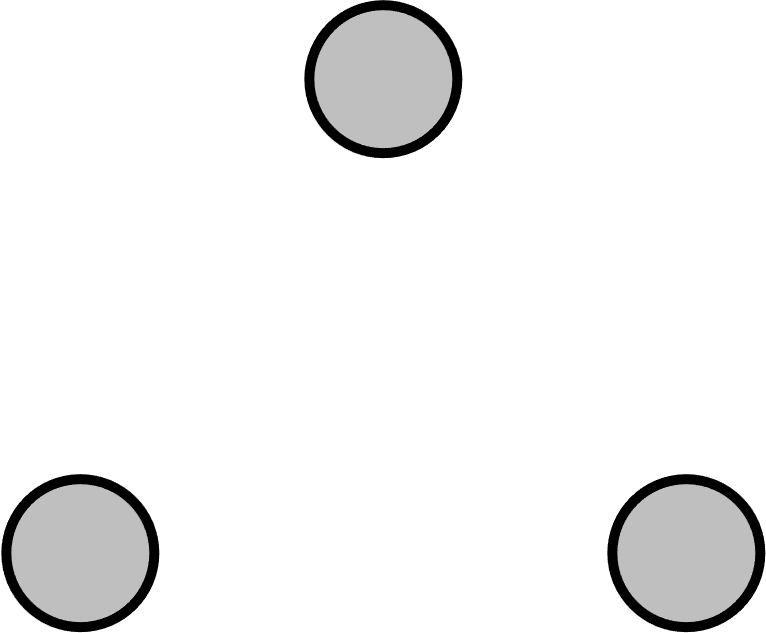
\includegraphics[width = \textwidth]{Images/Open_Triad.png}
\caption{Open triad.}
\end{subfigure}
\hspace{2em}
\begin{subfigure}[b]{0.25\textwidth}
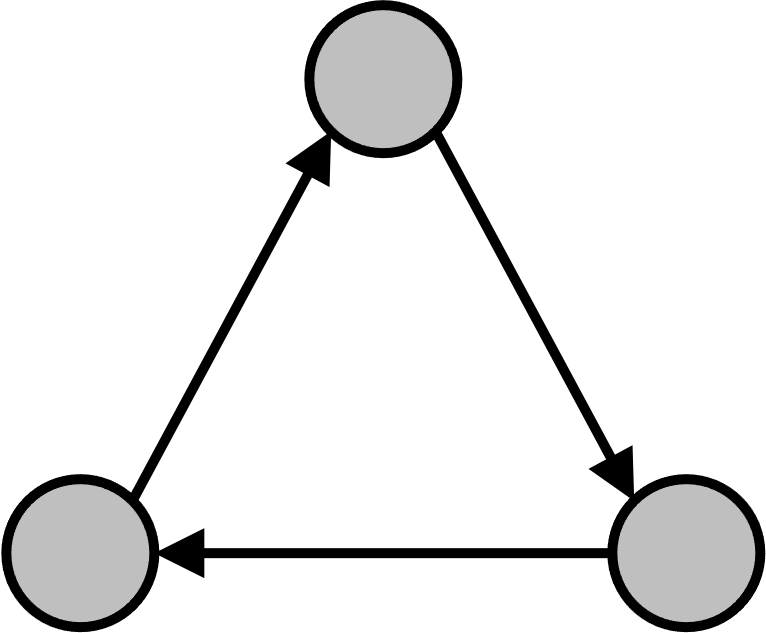
\includegraphics[width = \textwidth]{Images/C_Closure.png}
\caption{Cyclic closure.}
\end{subfigure}
\hspace{2em}
\begin{subfigure}[b]{0.25\textwidth}
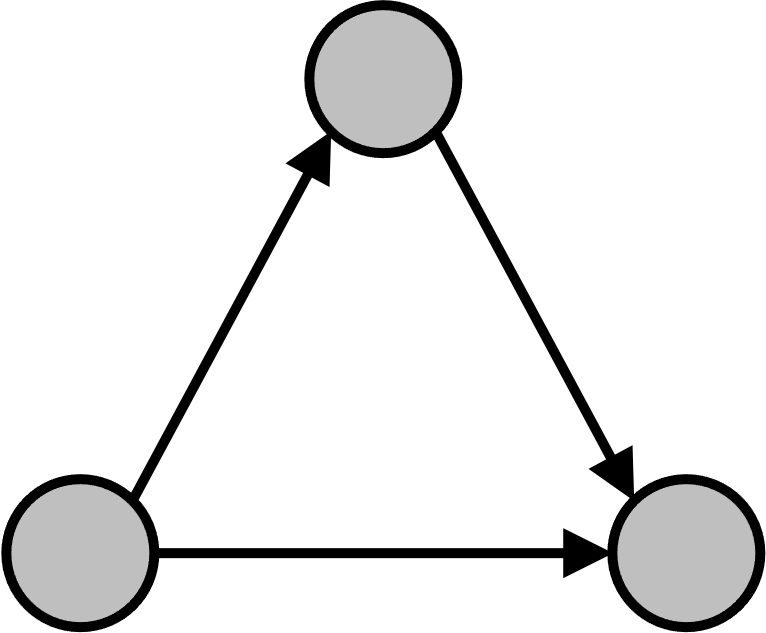
\includegraphics[width = \textwidth]{Images/T_Closure.png}
\caption{{Transitive closure.}}
\end{subfigure}
\includegraphics{}
\caption{Network closure measures the completeness of relational triads or triangles. Network closure creates the social conditions that build mutual trust\citep{coleman1990foundations}. There are two main types of closure: cyclic closure indicates generalised exchange, whereas transitive closure results in one actor benefiting more from exchanges than the other two actors. Empirical studies reveal that transitive closure is much more common than cyclic closure \citep{davis1967structure}.}
\label{fig:closure}
\end{figure}

\subsection{Reciprocal nature of trust}

Reciprocity is a crucial concept in social exchange and game theory and reflects a human tendency to return helpful or harmful acts in kind \citep{nowak2005evolution}. It is considered one indicator of trust in social networks \citep{blau1964exchange, rempel1985trust, lusher2012trust, cropanzano2016social}. According to social exchange theory, individuals act to maximise the potential of economic and social returns \citep{homans1961social, blau1964exchange}. A person does another a favour with a general expectation of some future non-binding return. Trust is more likely to develop between partners when exchange occurs without explicit negotiations or binding agreements. Under such conditions, the risk and uncertainty of exchange provide the opportunity for partners to demonstrate their trustworthiness \citep{molm2000risk}. Inadequate reinforcement or asymmetry in economic or social returns may result in the breakdown of trust \citep{homans1961social}. \medskip

Trust usually develops gradually over time through observations of past behaviour \citep{mayer1995integrative}. Achievement of trust at one level enables the development of trust at the next level and so on \citep{robert2009individual}. Swift trust is a presumptive form of trust that may explain trusting behaviour exhibited by members of temporary organisations\footnote{A temporary organisation is a \enquote{a temporally bounded group of interdependent organisational actors, formed to complete a complex task} \citep{burke2016temporary}, which is an apt description of an open innovation partnership}. Team members \enquote{suspend doubt} about the dependability of unknown others to accomplish a task \citep{germain2014role}. Influenced by their disposition towards trust, team members use \enquote{category-based information processing} to form an initial swift trust judgement by mentally placing others into a specific trust category. Team members adjust their trust beliefs according to fulfilled or unfulfilled expectations \citep{meyerson1996swift,robert2009individual}. \medskip

In game theory, the \enquote{prisoner's dilemma} is a game that explores the tension between individual self-interest and collective cooperation \citep{richards2001reciprocity}. Individuals or groups are assumed to be primarily motivated by self-interest. Modelling of the \enquote{prisoner's dilemma} shows that people can maximise their payoff through cooperative action based on simple reciprocity or \enquote{tit-for-tat} behaviour \citep{axelrod1980effective,axelrod1981evolution}. Tit-for-tat involves cooperating with your partner on the first round, then adjusting your behaviour to match your partner's in subsequent rounds. If your partner cooperates reciprocally, you continue to cooperate. However, should they defect, you respond in kind by retaliating immediately against them. The assumption is that people who start with good intentions (e.g. by being nice, generous, or forgiving) are more likely to be cooperative \citep{blais1987epistemic,richards2001reciprocity, segal2007tit, fulmer2013trust}. People will not be inclined to share tacit knowledge unless they see some personal advantage to do so \citep{yang2006knowledge, singh2019territoriality}. Swift trust and tit-for-tat behaviour have much in common \citep{fulmer2013trust}. People tend to respond favourably to swift trust, which contributes to positive working relationships. High-trusting temporary organisations are more likely to exhibit high-performance \citep{ashleigh2007trust}. Swift trust is vital in temporary organisations because it substitutes the traditional mechanisms of control and coordination found in established organisational hierarchies \citep{kasper2001communicating}. \medskip

Trust is a multidimensional construct. We can measure the extent to which individuals trust others. However, when we combine individual trust perceptions with other trust indicators, e.g. the level of reciprocity and closure in knowledge exchange networks, we start to see trust in a more holistic light. Hence, \bigskip

\begin{tcolorbox}
\textit{\textbf{Proposition 4a:} Reciprocity and closure in tacit knowledge exchange networks indicate high levels of trust in open innovation partnerships.}
\end{tcolorbox}

\section{Power}

As noted previously, two contrasting views of power dominate the literature: \enquote{power as domination}, otherwise referred to as \enquote{power-over}, and \enquote{power as empowerment}, also known as \enquote{power-to} \citep{haugaard2012rethinking}. This section explores how both forms of power may moderate tacit knowledge sharing in terms of structuration theory, power-dependence theory, and self-determination theory. 

\subsection{Power of tacit knowledge}

According to \citeauthor{giddens1984constitution}'s \citeyearpar{giddens1984constitution} structuration theory, agents derive their power from existing social structures that enable them to exercise power over others or afford them power to intervene in specific social situations. \citet{giddens1984constitution} considers \enquote{power-over} to be a subset of \enquote{power to}. For him, \enquote{power-to} is a transformative capacity that can change practices or structures. He sees \enquote{power-to} as something that resides in the \enquote{knowledgeability} of actors who know exactly what to do in different social contexts (what \citet{polanyi1966logic} refers to as \enquote{tacit knowing}). This aligns with the thinking of \citet{foucault1980power}, who argues power is knowledge and is inherent in all social relations where people negotiate meaning in terms of accepted forms of knowledge, scientific understanding, and truth \citep{diamond1988foucault}.\medskip

Tacit knowledge is a tremendous source of personal power, especially for those lower down the organisational hierarchy \citep{bordum2002tacit,gourlay2002tacit}. Attempts by organisations to codify the tacit knowledge embodied in their employees may be seen as a way of neutralising this power \citep{schultze2004knowing,singh2019territoriality}. By applying their tacit knowledge, people are exercising \enquote{power-to} bring about change \citep{schultze2004knowing,lam2014tacit}. In other words, tacit knowledge lies at the very heart of the structure versus agency debate \citep{lam2000tacit,lam2014tacit}. 

\subsection{Power as a relational construct}

Both concepts of power-over and power-to treat power as a relational construct, where the distribution of power reflects the structure of exchange opportunities \citep{blau1964exchange,reagans2008knowledge,bonacich2009structural}. The power of one actor over another reflects the dependence of the second on the first for a valued resource \citep{emerson1962power}. Preferential attachment theory suggests actors prefer to attach to well connected actors over poorly connected actors \citep{barabasi1999emergence}. The consequence of this is that more central actors in a knowledge exchange network will acquire knowledge at a faster rate than others. This has implications for power-dependence relations. More central actors are able to exert much more influence because they have greater access to diverse knowledge and are able to dictate agendas \citep{bonacich1987power,foucault1980power}. \medskip

Power imbalances may lead those feeling disempowered or powerless to engage in cost-reduction or balancing operations \citep{emerson1962power}. Cost-reduction is a process in which a person adjusts his or her personal values to accommodate the demands of a powerful other. The less powerful person simply acquiesces to the more powerful other. Such behaviour does not alter the balance of power. Balancing operations, on the other hand, aim to shift the balance of power. For example, tensions generated by power inequality can result in network extension where power-disadvantaged actors may seek out new social connections to reduce their dependence on a given actor for valued resources \citep{cook2013social}. Other ways to balance power include motivational withdrawal or deference \citep{emerson1962power}. Balancing operations illustrate how the distinctive causal powers of both individuals and social structures interact to determine social outcomes \citep{loyal2001agency}. \medskip

\enquote{Power-to} can also be treated as a relational construct. Powerful actors can empower others through power sharing or delegating authority. Since powerful actors control who they share power with or delegate authority to, this may be perceived as a limited form of empowerment \citep{conger1988empowerment}. Power-over others has been identified as barriers to knowledge sharing \citep{riege2005three,suppiah2011organisational}. People in authority often serve as gatekeepers of knowledge to preserve or enhance their status \citep{cross2001beyond}. Actors who do not award status to more powerful actors are likely to withhold their tacit knowledge from them \citep{cabrera2006determinants}. However, actors may be more willing to seek out tacit knowledge from more central actors whose power stems from deference relating to their expertise. Alternatively, actors are more likely to share tacit knowledge with others at a similar level of power as them \citep{cabrera2006determinants}. \medskip

\citet{todorova2007absorptive} claim that power relations inside the firm moderate the assimilation and transformation of knowledge, while power relations between partners moderate the relationship between absorptive capacity and competitive advantage. \citet{easterby2008absorptive} observe that political acts by brokers affect access to external knowledge, while diffusion of knowledge within a firm depends on the extent to which employees are empowered. 

\subsection{Power as a motivational construct}

Earlier it was stated that individuals are motivated to achieve greater self-efficacy to better manage prospective situations they may find themselves in. The quest for self-efficacy drives individual learning, much of which is achieved by observing how others behave or act \citep{bandura1994self}. Individuals empower themselves by accumulating tacit knowledge. The know-how and expertise helps them cope with the physical and social demands of the environment. Individuals who share their hard-earned know-how or expertise are empowering others. Any strategy that undermines the self-efficacy of organisational members will increase their feelings of powerlessness. This speaks directly to the \enquote{agency versus structure} debate, i.e. power-to promotes human agency whereas structure is often about exercising power-over others.

\subsection{Relationship between trust and power}

In a power-dependence relation, a powerful actor can reasonably expect the less powerful other to place a high value on their exchange relationship because the less powerful person does not have many options to access this resource elsewhere \citep{emerson1962power}. \citet{schilke2015power} find that power-disadvantaged actors tend to be more trusting than powerful actors. They suggest that, with increasing dependence, power-disadvantaged actors invest more cognitive resources in processing trust-related information that becomes available in an exchange than more powerful actors. Power-disadvantaged actors are likely to see the more powerful other as trustworthy to avoid anxiety stemming from their feelings of dependence. \citet{schilke2015power} suggest hope and perceived benevolence feature strongly in the trust decisions of power-disadvantaged. \medskip

Tacit knowledge is a tremendous source of personal power and deference. Resisting the formalisation of tacit knowledge can help maintain personal power \citep{schultze2004knowing}. While a power-disadvantaged actor might be less inclined to share their tacit knowledge with a more powerful other, they may end up doing so anyway to reduce anxiety. A more powerful actor may be less inclined to trust others with their tacit knowledge \citep{schilke2015power}. Hence, \bigskip

\begin{tcolorbox}
\textit{\textbf{Proposition 4b:} Who people choose to empower with their know-how depends on how much they trust the receiver to use their know-how in mutually beneficial ways.} 
\end{tcolorbox}

\section{Summary}

Conceptualising an open innovation partnership as a temporary knowledge network allows one to use social network analysis to assess knowledge sharing practices in meaningful ways. Extracting value from the knowledge network depends on the absorptive capacity of partners. Whereas experiential knowledge is a vital component of absorptive capacity, applying knowing in practice also builds absorptive capacity. Applying knowing in practice requires good quality relationships. Brokers not only facilitate access to diverse sources of knowledge and expertise, but they also can help others make sense of unfamiliar knowledge. Brokers occupy powerful positions as they can control access to knowledge. However, they can also empower others by giving them access to knowledge. Patterns of brokerage can reveal much about power relations in open innovation partnerships. \medskip

The main argument of this chapter is that the quest for tacit knowledge drives agency. Agents acquire tacit knowledge to not only satisfy an innate need for competence, but also to gain sufficient power to maintain or enhance their autonomy and to influence agendas and enact change. This has implications in terms of structure versus agency. Two key assumptions guide our thinking going forward: First, agency lies at the heart of tacit knowledge sharing. Second, innovation depends on the application of know-how in new or different contexts. These two assumptions suggest that informal structure is an essential feature in any open innovation partnership. We can describe this informal structure as an intentional community of practice. One can argue that successful open innovation depends on the emergence of informal structure and how well this operates as an intentional community of practice. \medskip

Effective open innovation structures are those that recognise people are driven by a need for competence. Because tacit knowledge is a source of personal power, individuals are going to be very selective in who they choose to share their tacit knowledge with. They are unlikely to surrender their hard-earned tacit knowledge if the costs of doing so outweigh the benefits. Individuals are less likely to reveal their tacit knowledge to those they do not trust or those who have power over them. With respect to open innovation, formal structures and prevailing culture in each partner organisation are likely to influence how individual participants interact across organisational boundaries. Given the important role of tacit knowledge in innovation, open innovation partnerships must be structured in ways that promote personal agency. Participants need to be able to choose who they share their tacit knowledge with. They are unlikely to share their tacit knowledge with others if power-relations are imbalanced. Participants need to work hard and building and maintaining trust, not only at an interpersonal level, but at the organisational level as well. Failure to do so will limit the flow of tacit knowledge. \medskip

How well open innovation partnerships function in practice is determined not so much by formal structures and prevailing cultures, but by the actions of individual participants. One may argue that open innovation success depends on the willingness of participants to share or seek out tacit knowledge. This willingness is moderated by personal levels of autonomous motivation, disposition to trust, and power relations in different social contexts. A better understanding of how people are motivated to share their know-how may contribute to more effective knowledge management practices in open innovation.\medskip

The seven propositions developed in this chapter are listed in Table \ref{tab:sum_props} and guide the thinking in the following chapters. The next chapter explains the methodology used to assess how motivation, trust, and power shape tacit knowledge sharing ties in open innovation partnerships. It includes justifications for embracing a critical realist worldview and need for a case-based mixed-method research design.

\begin{table}[]
\centering
\caption{List of propositions developed in Chapter 2.}
\label{tab:sum_props}
\resizebox{\textwidth}{!}{%
\begin{tabular}{@{}c p{12cm}@{}}
\toprule
Proposition & Statement \\ \midrule
1a & Open innovation requires practitioners to connect across organisational and disciplinary boundaries so they can apply their know-how in novel ways. \\
1b & Reducing cognitive distance between open innovation partners requires significant social  interaction to support learning and the application of knowledge in practice. \\
2a & Successful open innovation requires a combination of skilled brokerage that leads to network closure. \\
3a & Formal structures inhibit tacit knowledge exchange in open innovation partnerships. \\
3b & Innate needs and subjective norms moderate individual willingness to seek out or share tacit knowledge. \\
4a & Reciprocity and closure in tacit knowledge exchange networks indicate high levels of trust in open innovation partnerships. \\
4b & Who people choose to empower with their know-how depends on how much they trust the receiver to use their know-how in mutually beneficial ways. \\ \bottomrule
\end{tabular}%
}
\end{table}